%\documentclass[manuscript]{aastex}
%\documentclass[iop,useAMES,usenatbig]{emulateapj}
\documentclass[apj]{emulateapj}

\shorttitle{Simultaneous multi-band transits of WD1145+017}
\shortauthors{Zhou et al.}


%%% packages
\usepackage{graphicx}
\usepackage{amsmath}
\usepackage{amssymb}
\usepackage{xspace}
\usepackage{array}
\usepackage{natbib}
%bibliographystyle{apj}


{\renewcommand{\arraystretch}{4}%

\newcommand{\myemail}{george.zhou@cfa.harvard.edu}


\begin{document}

\title{Simultaneous infrared and optical observations of the transiting debris cloud around WD1145+017}

\author{G. Zhou\altaffilmark{1},
L.~Kedziora-Chudczer\altaffilmark{2,3},
J.~Bailey\altaffilmark{2,3},
J.P.~Marshall\altaffilmark{2,3},
D.D.R.~Bayliss\altaffilmark{4},
C.~Stockdale\altaffilmark{5},
P.~Nelson\altaffilmark{6},
T.G.~Tan\altaffilmark{7},
J.E.~Rodriguez\altaffilmark{8},
C.G.~Tinney\altaffilmark{2,3},
D.~Dragomir\altaffilmark{9},
K.~Colon\altaffilmark{10},
A.~Shporer\altaffilmark{11},
J.~Bento\altaffilmark{12},
R.~Sefako\altaffilmark{13},
K.~Horne\altaffilmark{14}, and
W.~Cochran\altaffilmark{15}}

\altaffiltext{1}{Harvard-Smithonian Center for Astrophysics, 60 Garden St., Cambridge, MA 02138, USA \email{\myemail}}
\altaffiltext{2}{School of Physics, University of New South Wales, Sydney, NSW 2052, Australia}
\altaffiltext{3}{Australian Centre for Astrobiology, University of New South Wales, Sydney, NSW 2052, Australia}
\altaffiltext{4}{Observatoire Astronomique de l'Universit\'{e} de Gen\`{e}ve, 51 ch. des Maillettes, 1290 Versoix, Switzerland}
\altaffiltext{5}{Hazelwood Observatory, Victoria, Australia}
\altaffiltext{6}{Ellinbank Observatory, Victoria, Australia}
\altaffiltext{7}{Perth Exoplanet Survey Telescope, Western Australia, Australia}
\altaffiltext{8}{Department of Physics and Astronomy, Vanderbilt University, 6301 Stevenson Center, Nashville, TN 37235, USA}
\altaffiltext{9}{The Department of Astronomy and Astrophysics, University of Chicago, 5640 S Ellis Ave, Chicago, IL 60637, USA}
\altaffiltext{10}{NASA Ames Research Center, M/S 244-30, Moffett Field, CA 94035, USA}
\altaffiltext{11}{Jet Propulsion Laboratory, California Institute of Technology, 4800 Oak Grove Drive, Pasadena, CA 91109, USA}
\altaffiltext{12}{Research School of Astronomy and Astrophysics, the Australian National University, Canberra, ACT 2611, Australia}
\altaffiltext{13}{SAAO, P O Box 9, Observatory 7935, South Africa}
\altaffiltext{14}{SUPA Physics and Astronomy, University of St. Andrews, KY16 9SS, Scotland, UK}
\altaffiltext{15}{McDonald Observatory, The University of Texas, Austin, TX 78712, USA}
%\altaffiltext{16}{Laboratoire d'astrophysique de Marseille, Technople de Marseille-Etoile 38, rue Fr\'{e}d\'{e}ric Joliot-Curie, 13388 Marseille cedex 13, France}


\begin{abstract}
We present multi-wavelength photometric monitoring of the WD 1145+017, a white dwarf exhibiting periodic dimming events interpreted to be the transits of orbiting, evaporating planetesimals. Our observations range from the $g'$ band in the optical to the near-infrared $J$ band, and record multiple transit events with depths ranging from $\sim 20$\% to 50\%. Simultaneous near-infrared and optical observations of the largest transit were obtained at two epochs with the Anglo-Australian Telescope and three optical facilities. These observations revealed no measurable difference in transit depths for multiple photometric pass bands, allowing us to place a $2\sigma$ lower limit of $0.8\,\mu\mathrm{m}$ on the grain size in the putative transiting debris cloud. Large variations in the transit depths were seen over the one month temporal baseline, confirming the highly variable nature of the system. 
\end{abstract}

\keywords{keywords}

\section{Introduction}
\label{sec:introduction}

The transit events detected around WD 1145+017 may be the first direct evidence for in-falling planetesimals polluting the atmosphere of a white dwarf. Photometric monitoring of the white dwarf by the \emph{K2} mission revealed a series of asymmetric transits, with depths of $\sim 40$\% and periods of 4.5 to 4.9 hours \citep{2015Natur.526..546V}. The white dwarf also shows heavy element pollution in its spectra, and infrared excess in its spectral energy distribution \citep{2015Natur.526..546V,2016ApJ...816L..22X}. In addition, \citet{2016ApJ...816L..22X} reported that broadened absorption lines from heavy elements were superimposed on the sharp atmospheric metal lines, suggesting the presence of circumstellar material with orbital velocities of $\sim 300\,\mathrm{km\,s}^{-1}$ surrounding the host star. Subsequent ground-based photometric monitoring has revealed a series of semi-periodic dimming events \citep{2015Natur.526..546V,2015arXiv151006434C,2016ApJ...818L...7G,2016MNRAS.tmp..406R,2016arXiv160308823A}. Multiple events are often seen within a given period with depths that vary by as much as 60\%, and with life-times as short as days. These observations have been interpreted as a series of transits by fragments of a debris cloud surrounding WD 1145+017, and are perhaps indicative of dust originating from evaporating planetesimals. Some 30-50\% of white dwarfs have spectra that exhibit pollution by heavy elements \citep[e.g.][]{2003ApJ...596..477Z,2010ApJ...722..725Z,2014A&A...566A..34K}, while 1-3\% of white dwarfs have a detectable infrared excess suggestive of debris disks \citep[e.g.][]{2003ApJ...584L..91J,2007ApJS..171..206M,2009ApJ...694..805F,2011MNRAS.417.1210G,2011ApJS..197...38D}. WD 1145+017 is the first white dwarf found to exhibit probable transit events originating from its circumstellar material, and gives us an unique opportunity to study the dust properties before it is accreted onto the star. 

If a significant part of the transiting debris cloud is optically thin, then we should expect the depth and shape of the transits to be wavelength dependent. \citet{2015arXiv151006434C} reported a series of simultaneous $V$ and $R$ band light curves from May 2015, finding no depth differences in the transits. \citet{2016arXiv160308823A} have reported OSIRIS spectrophotometric observations from the 10.4\,m Gran Telescopio Canarias. These spanned $0.48-0.92\,\mu\mathrm{m}$, and detected a series transits ranging from 25\% to 40\%, but which displayed no change in transit depth across multiple wavelength bins. This lack of wavelength-depth dependence in the optical excludes the presence of particles smaller than $ 0.5\,\mu \mathrm{m}$ in any debris cloud. 

Despite the faintness of WD 1145+017 ($g=17.029$, $J=17.504$), the deep transits make it an excellent target for multi-wavelength follow-up observations. In this study, we extend the wavelength baseline to the near-infrared with $J$ band light curves obtained at the Anglo-Australian Telescope (AAT) over multiple nights spanning a baseline of one month. Two of these near-infrared transits have been observed simultaneously in the optical in coordination with other facilities. This, as well as subsequent optical follow-up observations, allowed us to monitor for wavelength-depth dependencies and evolutions in the transits about the white dwarf.

\section{Observations and reduction}
\label{sec:observations}

Photometric imaging observations have been obtained with multiple telescopes: $J$ band infrared observations with the AAT; optical observations 
obtained simultaneously with some of this infrared data using a suite of small telescopes across Australia; and follow-up $g'$ band observations with the Las Cumbres Observatory Global Telescope (LCOGT) network. These observations are summarised in Table~\ref{tab:observations}, and their acquisition and analysis is described in full below.

\begin{table*}
\centering
\caption{\label{tab:observations}List of observations}
\begin{tabular}{lllrr}
\hline\hline
Facility & Dates & UT Time & Photometric band & Exposure time (s) \\
\hline
AAT+IRIS2 3.9\,m & 2016-02-16 & 13:13 -- 18:16 & $J$ & 30 \\
AAT+IRIS2 3.9\,m & 2016-02-17 & 16:27 -- 18:37 & $J$ & 30 \\
AAT+IRIS2 3.9\,m & 2016-02-19 & 16:27 -- 18:34 & $J$ & 30 \\
AAT+IRIS2 3.9\,m & 2016-02-20 & 16:59 -- 18:30 & $J$ & 30 \\
AAT+IRIS2 3.9\,m & 2016-02-21 & 15:57 -- 18:34 & $J$ & 30 \\
Hazelwood 0.32\,m & 2016-03-19 & 10:36 -- 18:18 & Clear & 300 \\
AAT+IRIS2 3.9\,m & 2016-03-19 & 11:15 -- 16:26 & $J$ & 30 \\
Ellinbank 0.32\,m & 2016-03-19 & 12:25 -- 16:48 & Clear & 180 \\
Hazelwood 0.32\,m & 2016-03-20 & 09:59 -- 13:15 & Clear & 300 \\
AAT+IRIS2 3.9\,m & 2016-03-20 & 11:00 -- 17:27 & $J$ & 30 \\
Ellinbank 0.32\,m & 2016-03-20 & 11:28 -- 17:02 & $R$ & 240 \\
PEST 0.30\,m & 2016-03-19 & 14:53 -- 20:28 & $V$ & 240 \\
LCOGT 1\,m Sutherland & 2016-03-25/26 & 18:36 -- 02:00 & $g'$ & 150 \\
LCOGT 1\,m Cerro Tololo & 2016-03-26 & 00:11 -- 05:11 & $g'$ & 150 \\
LCOGT 1\,m Sutherland & 2016-03-28/29 & 18:36 -- 01:46 & $g'$ & 150 \\
\hline
\end{tabular}
\end{table*}

\subsection{AAT $J$ band observations}
\label{sec:obs_aat}

We obtained near-infrared light curves for WD 1145+017 using the IRIS2 camera \citep{2004SPIE.5492..998T} on the 3.9\,m AAT, located at Siding Spring Observatory, Australia. IRIS2 is a near-infrared camera, with a $1\,\mathrm{K} \times 1\,\mathrm{K}$ HAWAII-1 HgCdTe infrared detector, read out over four quadrants, achieving a field of view of $7.7' \times 7.7 '$ and a pixel scale of $0.4486''\,\mathrm{pixel}^{-1}$. Our observations were performed in the $J$ band using a 30\,s integration time and read out in double-read mode. A photometric precision of $\sim 10\mathrm{\%}$ was achieved on each exposure. The observing strategy, data reduction, and photometry extraction used followed the procedures described in \citet{2014MNRAS.445.2746Z,2015MNRAS.454.3002Z}. The one exception being that, due to the faintness of the target star, these observations were not defocused. Each sequence of light curves was obtained with the telescope locked to a nearby guide star, with the observer applying small manual offsets every $\sim 10$ minutes to ensure to ensure the target and reference stars stayed on the same pixel throughout. Dithered sequences bracketing these `stare' observations provide the flat-field and sky background corrections. Photometry of the target and reference stars were extracted in circular apertures at a series of radii, and background estimated in annuli around each aperture. The image coordinate matching and photometric extraction are performed using the \emph{FITSH} package \citep{2012MNRAS.421.1825P}. Reference photometry is performed against a selection of stable reference stars. Six extraction apertures of fixed radii were used, with the aperture that yields the lowest out-of-transit scatter selected. The transit depth analyses presented in Section~\ref{sec:lightcurve_model} were tested against all extraction apertures. The scatter in derived transit depths due to aperture selection is smaller than the statistical error in each aperture by a factor of four or more. 

Two full nights of AAT+IRIS2 observations were obtained simultaneously with optical observations from a suite of small telescopes on 2016-03-19 and 2016-03-20. Poor weather meant only segments of light curves could be recovered on 2016-03-19. However conditions were photometric on 2016-03-20. These observations are plotted in Figures~\ref{fig:lc_20160319} and \ref{fig:lc_20160320}. 

In addition, observations of WD 1145+017, without simultaneous optical observations, were obtained over five nights of 2016-02-16,17,19,20,21. These provided a longer-term baseline to examine the near-infrared evolution of the debris cloud. These light curves are shown in Figure~\ref{fig:lc_201602}.

\begin{figure*}
    \vspace{5mm}
    \centering
    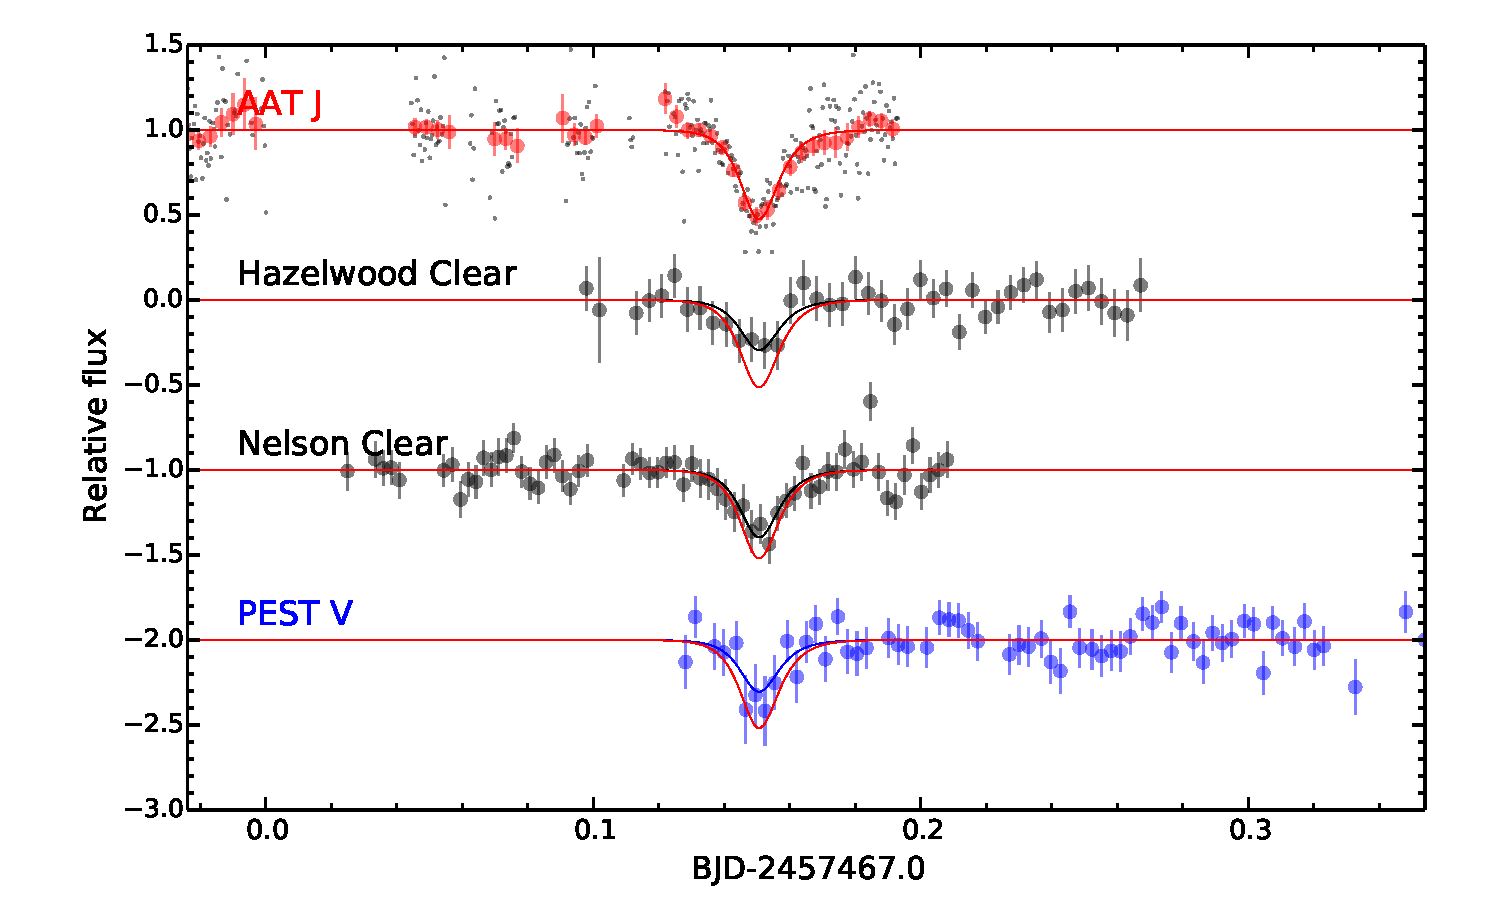
\includegraphics[width=15cm]{plots/20160319.eps}
    \caption{The light curves of WD 1145+017 from 2016-03-19, simultaneously observed by the AAT in the infrared $J$ band, and by a series of small telescopes in the optical. The individual AAT observations are plotted in grey, and the 5 min binned light curve in red. The error bars represent the mean uncertainty of the points within the bin, scaled by the square root of the number of points per bin. The light curves of the optical facilities are shown at their native cadence. The shaded areas represent the $1\sigma$ region in the model fit. The solid lines show the best fit models according to Equation~\ref{eq:model}. The optical light curves have their respective model fits and the model fits to the AAT $J$ band light curve (red) over-plotted for comparison.}
    \label{fig:lc_20160319}
\end{figure*}

\begin{figure*}
    \vspace{5mm}

    \centering
    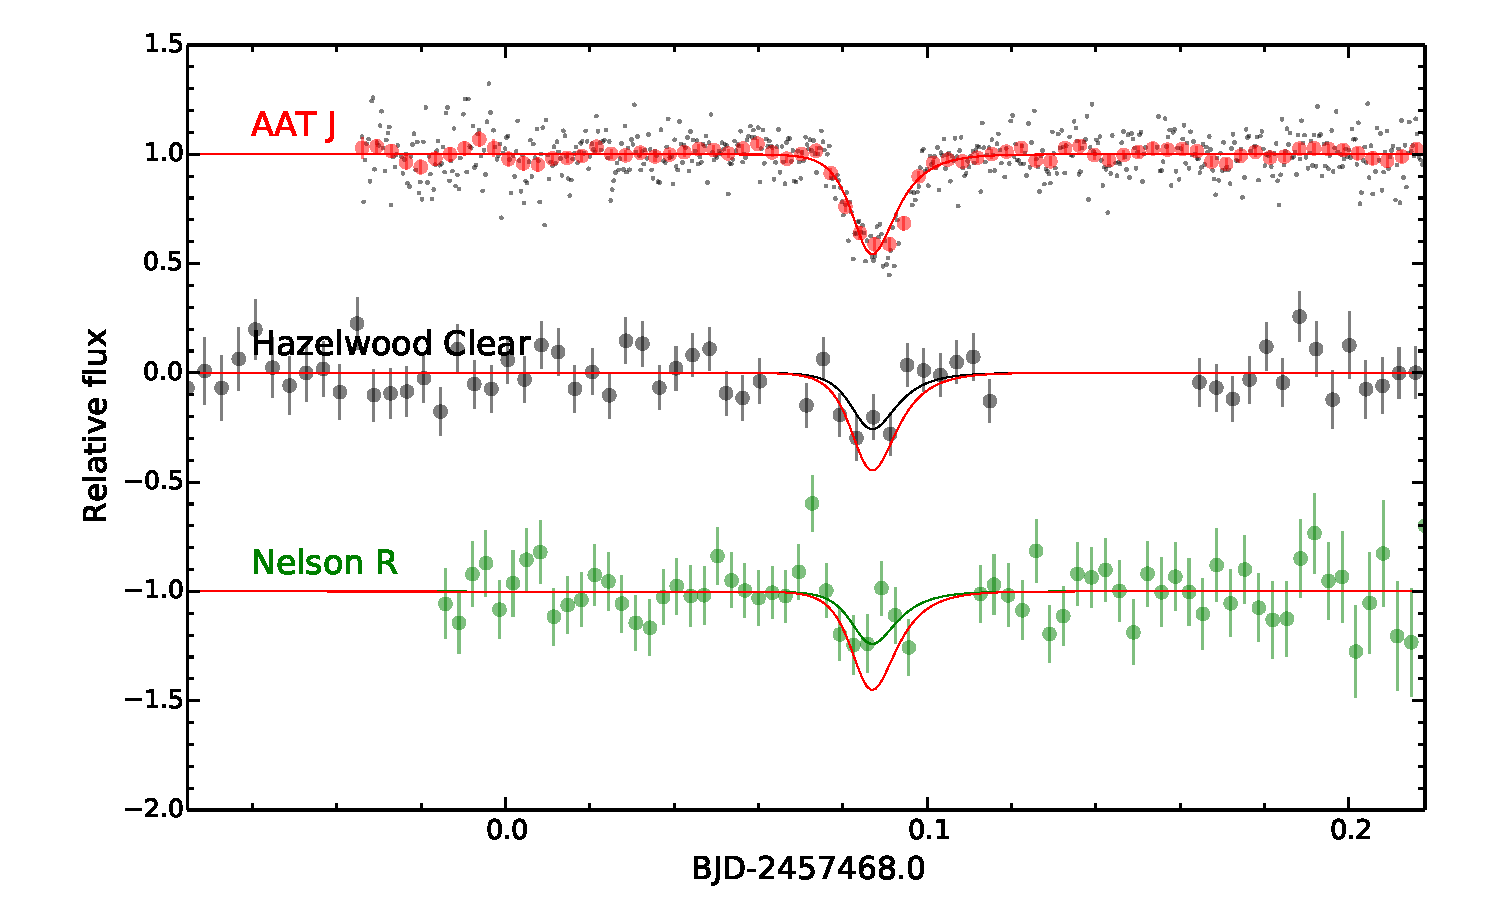
\includegraphics[width=15cm]{plots/20160320.eps}
    \caption{The light curves of WD 1145+017 from 2016-03-20, simultaneously observed in the infrared by AAT and in the optical by a series of small telescoeps. See Figure~\ref{fig:lc_20160319} for description.}
    \label{fig:lc_20160320}
\end{figure*}


\begin{figure*}
    \vspace{5mm}
    \centering
    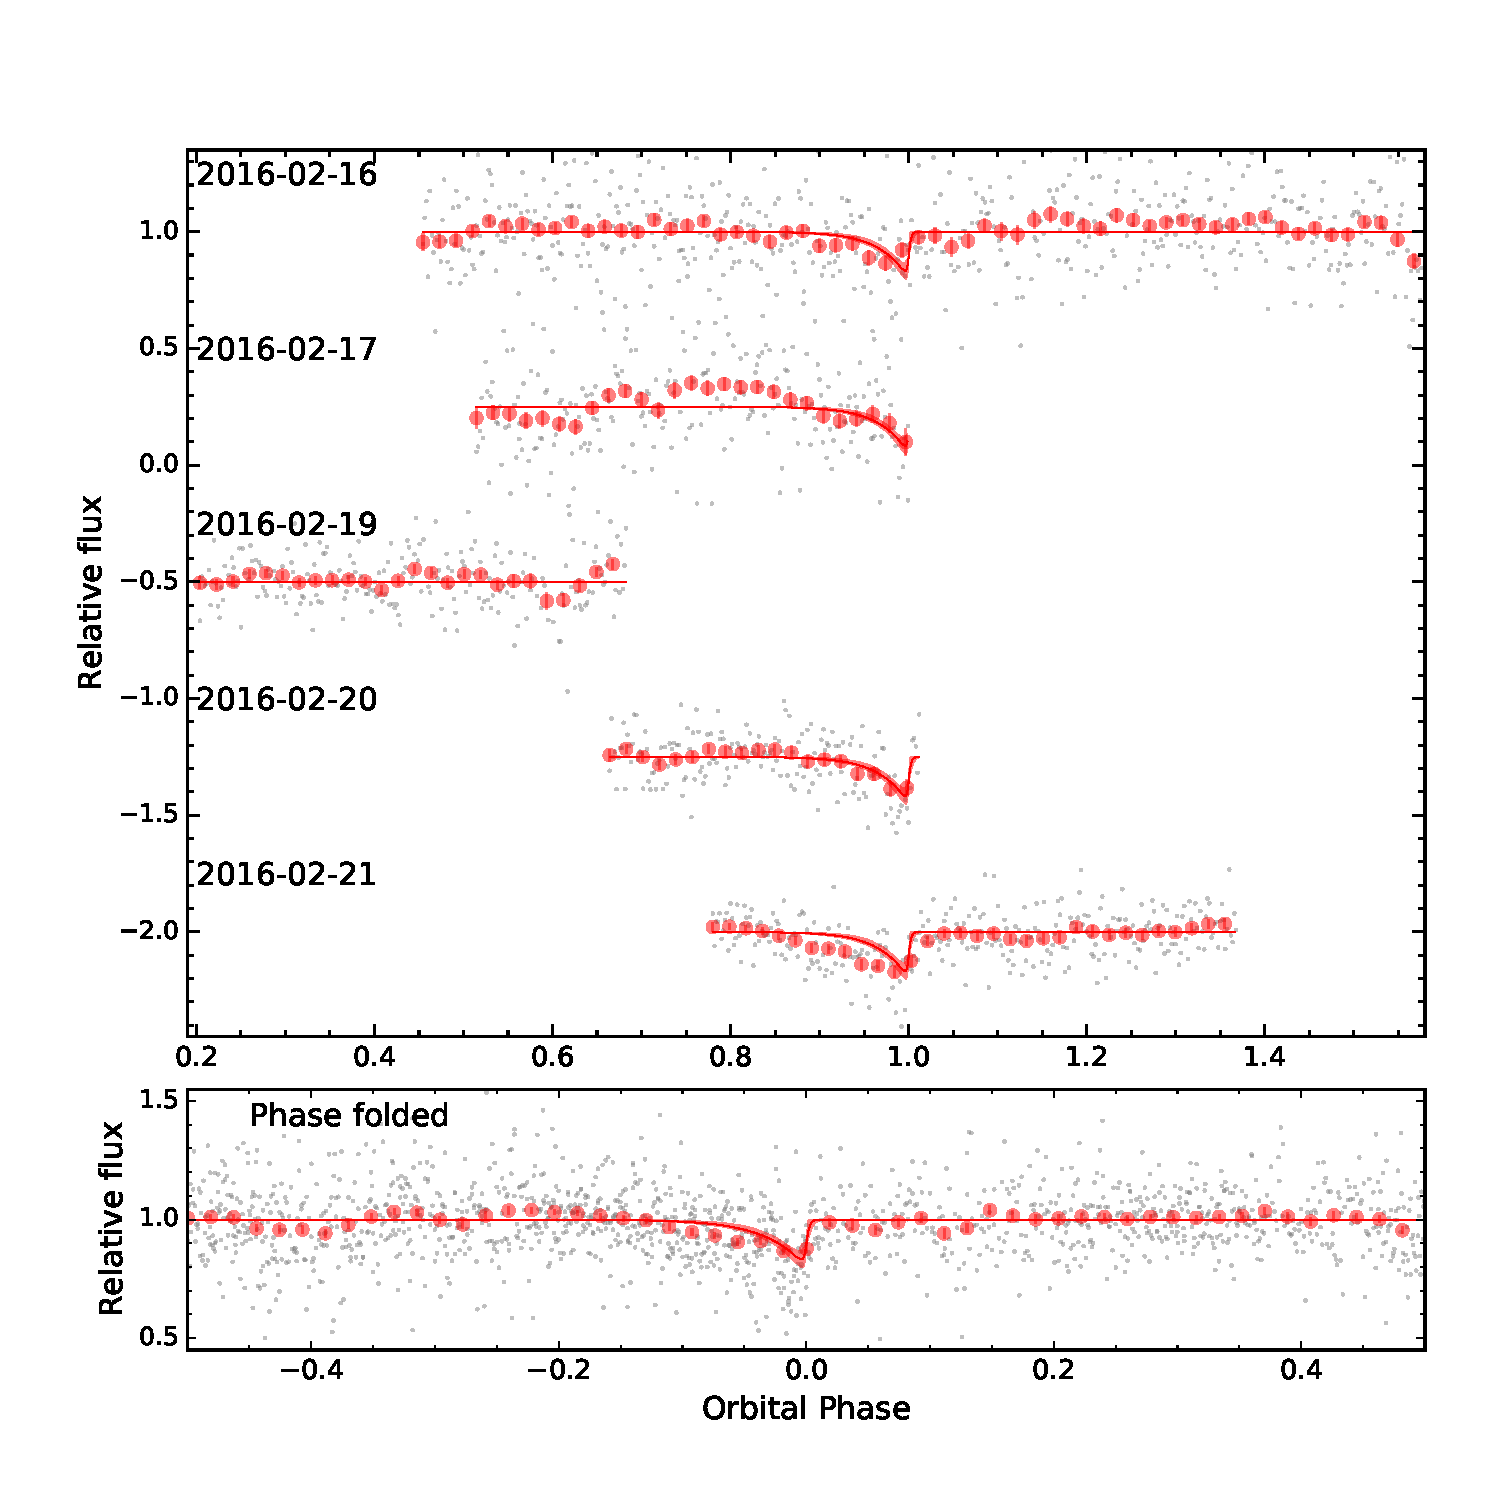
\includegraphics[width=15cm]{plots/AAT_feb.eps}
    \caption{WD 1145+017 was monitored over five nights in February 2016 by the AAT in the near-infrared $J$ band. Two full transit events were captured during this period. The top panel shows the light curve from each night, with individual points plotted in grey, and the 5 min binned light curve in red. The shaded region represents the $1\sigma$ regime for the allowed models, assuming the transits can be described by a single model. The bottom panel shows the phase binned light curve and model.}
    \label{fig:lc_201602}
\end{figure*}


\subsection{Simultaneous optical observations}
\label{sec:simultaneous-optical}

Optical observations were obtained by multiple small telescopes across Australia on 2016-03-19 and 2016-03-20 simultaneously with the near-infrared photometry described in Section~\ref{sec:obs_aat}. 

Observations on these two nights were obtained with the 0.32\,m Planewave CDK telescope at Hazelwood Observatory, operated by Chris Stockdale in Victoria, Australia. The exposures were made with a SBIG ST8XME $1.5\mathrm{K}\times1 \mathrm{K}$ CCD detector, yielding a $18'\times12'$ field of view and a $0.73''/\mathrm{pixel}$ plate scale. Due to the faintness of the target, no filter was used. The setup is fully described in \citet{2015arXiv150908953R}.

Observations on the same two nights were also obtained at the Ellinbank observatory, Victoria, with the 0.32\,m Planewave CDK telescope, operated by Peter Nelson. The observations were obtained using a SBIG 3200 ME CCD camera, with a $2184\times1472$ detector, with a field of view of $20.2' \times 13.5'$ at a plate scale of 1.12''/pixel when read out at $2\times 2$ bin. The observations were performed over the optical (no filter) on 2016-03-19, and in the $R$ band on 2016-03-20. 

The Perth Exoplanet Survey Telescope (PEST) obtained observations on both nights. PEST is a fully automated observatory operating a 0.30\,m Meade LX200 Schmidt Cassegrain telescope, located in Perth, Western Australia and operated by T.G. Tan. The setup employs a SBIG ST-8XME detector, yielding a field of view of $31'\times 21'$ and a plate scale of $1.2''/\mathrm{pixel}$. Observations were performed in the $V$ band within an integration time of 240\,s on both nights. Unfortunately, the photometric precision from 2016-03-20 were not sufficient to provide useful constraints on the $V$ band transit, and are left out of the analysis. The PEST facility is also described in \citet{2015arXiv150908953R}.

Each set of images were bias- and dark-subtracted, and then flat field corrected. Light curves were extracted from the reduced frames using aperture photometry via the \emph{FITSH} package as described in Section~\ref{sec:obs_aat}. Reference photometry was obtained using a largely consistent set of reference stars (though not fully consistent due to differences in field centre and field-of-view). The light curves are shown in Figures~\ref{fig:lc_20160319} and \ref{fig:lc_20160320}. 


\subsection{Subsequent optical follow-up from LCOGT}
\label{sec:lcogt}

We obtained photometric observations using the LCOGT network within 5 days of our simultaneous infrared-optical campaign. The observations were performed on 2016-03-25 and 2016-03-28 using the 1\,m telescopes located at Sutherland observatory, South Africa, and on 2016-03-26 using an identical setup at Cerro Tololo observatory, Chile. An overlap of $\sim 2$ hours were available between the Cerro Tololo 2016-03-26 observations and that from Sutherland, allowing one transit to be captured simultaneously from both facilities. The observations were taken with the $4\mathrm{K} \times 4 \mathrm{K}$ SBIG STX-16803 camera, with a field of view of $15.8'\times 15.8'$ and a pixel scale of 0.464''/pixel when read out at $2\times 2$ bin. The observations were performed in the $g'$ band to provide a large wavelength baseline for comparison. The raw frames were processed with the automated LCOGT pipeline. Photometric extraction and reference photometry were extracted according to Section~\ref{sec:obs_aat}, via the \emph{FITSH} package. The light curves are shown in Figure~\ref{fig:lcogt}.

\begin{figure*}
    \vspace{5mm}
    \centering
    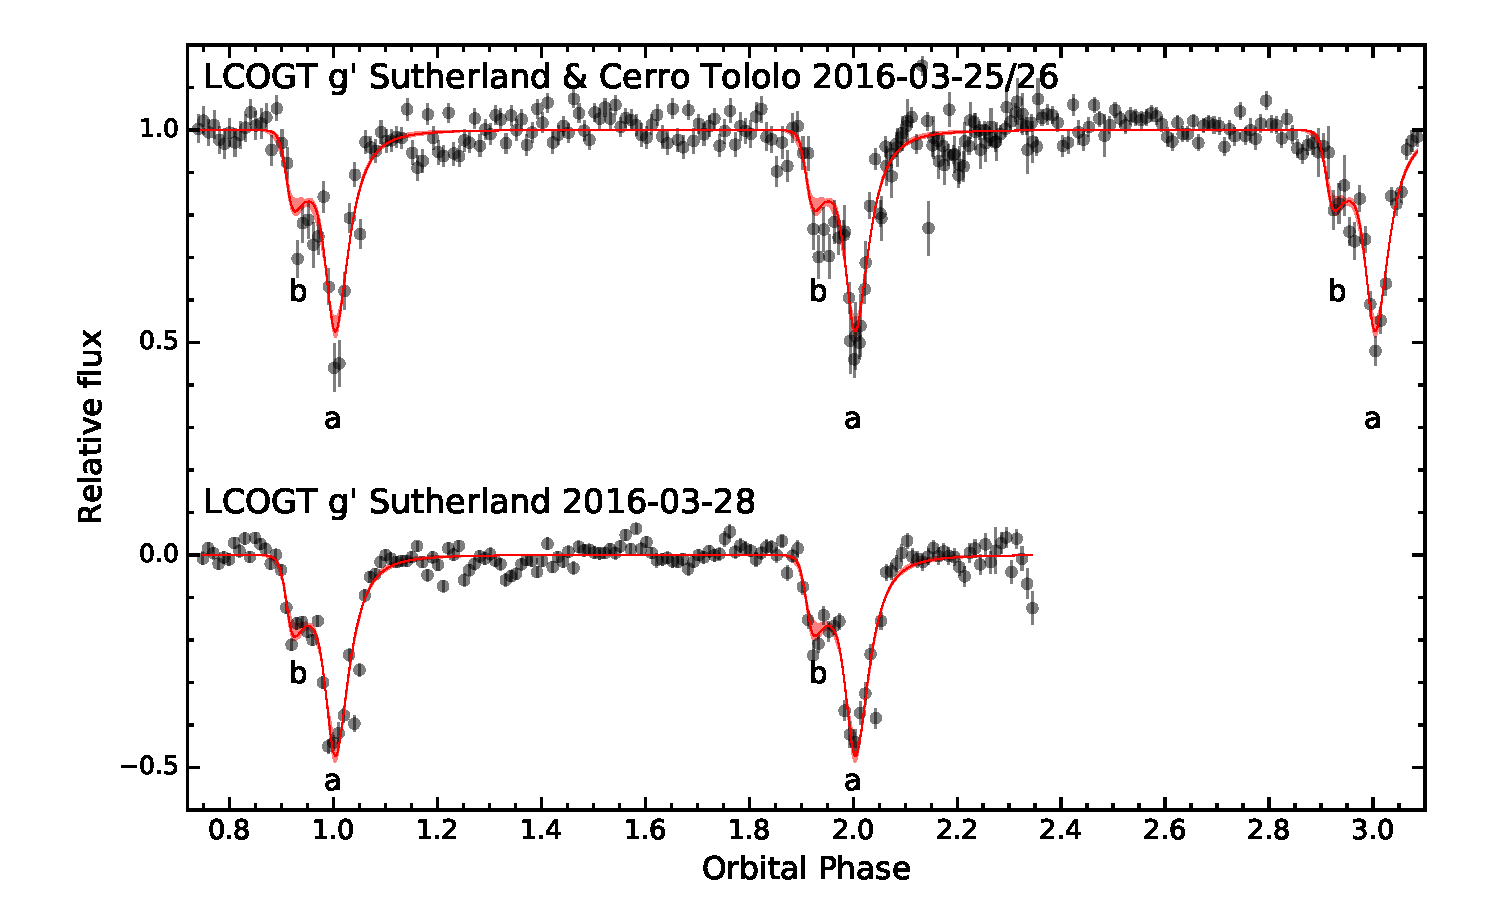
\includegraphics[width=15cm]{plots/lcogt.eps}
    \caption{$g'$ band light curves of WD 1145+017 on 2016-03-25/26 and 2016-03-28, 5 days after the set of simultaneous observations. Five main transit events were observed over the two nights, each transit event involved a large 40\% event, and an adjacent 20\% event. The light curves were fit with a doublet transit model, allowing for $\tau_0$ and period to be shared.}
    \label{fig:lcogt}
\end{figure*}



\section{Light curve analyses}
\label{sec:lightcurve_model}

\subsection{Global analysis of the simultaneous transit light curves}
\label{sec:simultaneous_lc}

The transits of WD 1145+017 evolve rapidly from orbit to orbit, and only simultaneous observations can give us a coherent analysis for the wavelength dependence of the transits. Following \citet{2014ApJ...784...40R} and \citet{2015arXiv151006434C}, we fit the transits with hyperbolic secant functions. Each transit is described by the parameters of transit depth $(C)$, reference transit centroid $(\tau_0)$, and characteristic timescales for ingress $(\tau_1)$ and egress $(\tau_2)$:
\begin{equation}
\label{eq:model}
  F(t) = 1 - C \left( \exp \left(\frac{-(t-\tau_0)}{\tau_1} \right) + \exp \left(\frac{t-\tau_0}{\tau_2} \right) \right)^{-1}\,.
\end{equation}
We assume a common shape for the light curve at different bands, such that the $\tau_0$, $\tau_1$ and $\tau_2$ parameters are shared across the transits observed on a given night. The depth $C$ is left independent for each band, allowing us to probe for transit depth differences.

The best fit parameters and associated uncertainties are derived via a Markov chain Monte Carlo analysis, using the \emph{emcee} \citep{2013PASP..125..306F} affine invariant ensemble sampler. Since the transits are of short duration, we account for the long exposure time of the follow-up optical light curves by integrating over the models for each exposure.

The observations and model fits for 2016-03-19 and 2016-03-20 are shown in Figure~\ref{fig:lc_20160319} and \ref{fig:lc_20160320}. The $1\sigma$ set of models allowed by the data are shaded for each plot. The resulting fit parameters are presented in Table~\ref{tab:simultaneous_params}. 

In each case the transit depth determined at each pass band is consistent (given the uncertainties) with a single value. Following \citet{2015arXiv151006434C}, the depth $D$ (the minimum of the transit) is given by: 
\begin{equation}
D = C \frac{\zeta^{\zeta/(1+\zeta)} }{1+\zeta}\,,
\end{equation}
where $\zeta = \tau_2/\tau_1$. Figure~\ref{fig:depth_hist} shows the posterior distribution for the derived depths of the transits at each band for each of the nights. We find no change to the transit depth and shape between the two nights, with $\tau_1 = 0.005\pm0.001$, $\tau_2 = 0.005\pm0.001$ on 2016-03-19 and $\tau_1 = 0.004\pm0.001$, $\tau_2 = 0.006\pm0.001$ on 2016-03-20. This is an important test, since the transit shape is known to change on a short time scale. The lack of detectable change allows us to combine the data from the two nights. 

We fit the data from both nights together, with all transits sharing the characteristic timescale parameters $\tau_1$ and $\tau_2$, and each band with an independent depth parameter $C$. The reference transit time $\tau_0$ and transit period $P$ are also fitted for, and shared globally. The resulting transit depth posteriors are plotted in Figure~\ref{fig:depth_hist}. No large difference in the transit depths were measured, with all depths agreeing to within $1\sigma$. The full set of derived parameter values are given in Table~\ref{tab:simultaneous_params}. Interestingly, we also find no significant asymmetry for the transits, differing from the transits one month earlier (Section~\ref{sec:single_band_lc}), and from many of the dimming events in literature \citep[e.g. FLWO transits from ][]{2015Natur.526..546V}. 

\begin{figure}
    \vspace{5mm}
    \centering
    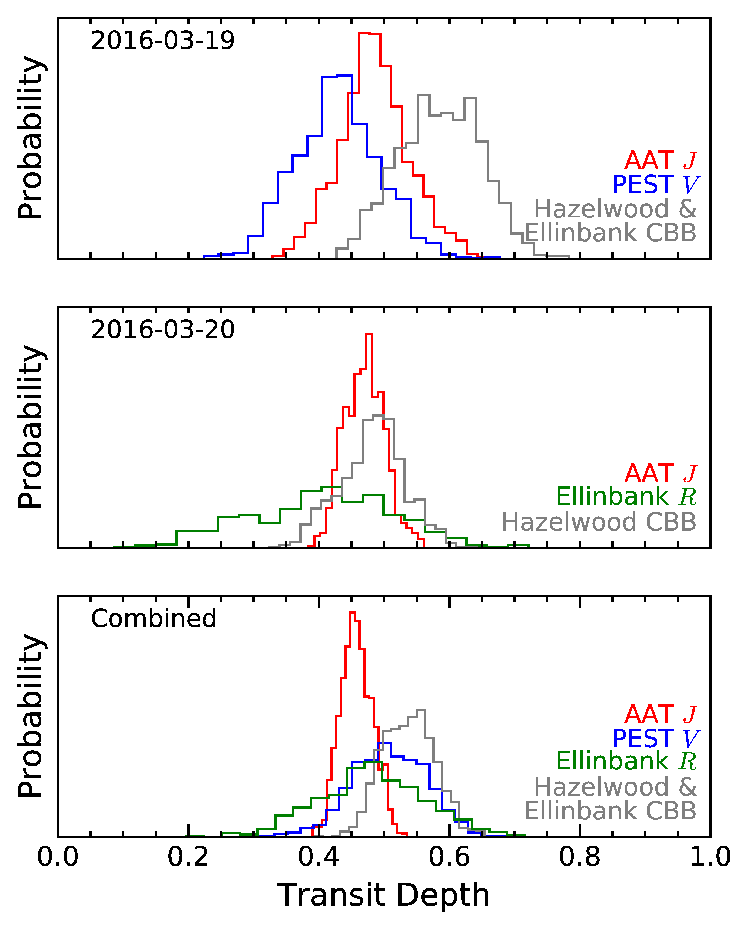
\includegraphics[width=7cm]{plots/depth_hist.eps}
    \caption{The transit depth $(D)$ posterior distribution for the transits simultaneously observed at the different photometric bands on 2016-03-19 (Top) and 2016-03-20 (Middle). The transits from each night were fit simultaneously, sharing the parameters governing the transit shape, but with different depths for each band. The transit depths agree between each photometric band, and between the two nights, at the $1\sigma$ level. The bottom panel shows the depth distribution derive from fitting the data from both nights simultaneously, with all transit shape parameters shared, and per-band transit depth independent. Again, the transit depths from each photometric band agree to within $1\sigma$.}
    \label{fig:depth_hist}
\end{figure}

\begin{table*}
\centering
\caption{\label{tab:simultaneous_params}Transit parameters from multi-band simultaneous observations}
\begin{tabular}{lrrr}
\hline\hline
Parameter & 2016-03-19 & 2016-03-20 & Combined\\
\hline
\textbf{Fitted parameters} & & & \\
$\tau_0$ (BJD-TDB) & $2457467.150_{-0.001}^{+0.001}$ & $2457468.086_{-0.002}^{+0.002}$ & $2457467.1495_{-0.0009}^{+0.0010}$\\
Period (d) & ... & ... & $0.1874_{-0.0001}^{+0.0001}$ \\ 
$\tau_1$ (d) & $0.0045_{-0.0009}^{+0.0011}$ & $0.0039_{-0.0006}^{+0.0007}$ & $0.0037_{-0.0004}^{+0.0004}$ \\
$\tau_2$ (d) & $0.0055_{-0.0007}^{+0.0009}$ & $0.006_{-0.001}^{+0.001}$ & $0.0056_{-0.0006}^{+0.0007}$ \\
$C_\mathrm{Clear}$ & $1.2_{-0.1}^{+0.1}$ & $0.9_{-0.1}^{+0.1}$ & $1.04_{-0.09}^{+0.08}$ \\
$C_V$ & $0.9_{-0.1}^{+0.1}$ & ... & $1.0_{-0.1}^{+0.1}$\\
$C_R$ & ... & $0.8_{-0.2}^{+0.2}$ & $0.9_{-0.1}^{+0.1}$ \\
$C_J$ & $0.95_{-0.09}^{+0.10}$ & $0.91_{-0.07}^{0.05}$ & $0.88_{-0.04}^{+0.06}$ \\
\textbf{Derived depths} && \\
$D_\mathrm{Clear}$ $(0.58_{-0.23}^{+0.19}\,\mu\mathrm{m})$ $^a$ & $0.59_{-0.06}^{+0.06}$ & $0.49_{-0.05}^{+0.04}$ & $0.54_{-0.04}^{+0.04}$ \\
$D_V$ $(0.52_{-0.05}^{+0.0.06}\,\mu\mathrm{m})$& $0.43_{-0.06}^{+0.06}$  & ... & $0.51_{-0.05}^{+0.05}$\\
$D_R$ $(0.64_{-0.07}^{+0.0.04}\,\mu\mathrm{m})$& ... & $0.41_{-0.12}^{+0.09}$ & $0.48_{-0.08}^{+0.08}$\\
$D_J$ $(1.24_{-0.07}^{+0.09}\,\mu\mathrm{m})$ & $0.48_{-0.04}^{+0.05}$ & $0.47_{-0.03}^{0.03}$ & $0.46_{-0.02}^{+0.03}$\\
\hline
\end{tabular}
    \begin{flushleft}
    $^a$ The wavelength centroid of the pass bands, accounting for detector efficiency, filter throughput, stellar flux, and atmospheric transmission. The error bars give the full width at half maximum of the transmission curve.\\
    \end{flushleft}
\end{table*}

\subsection{Light curves from single-band observations}
\label{sec:single_band_lc}


In addition to the simultaneous set of multi-wavelength observations, we also obtained $J$ band AAT light curves during five nights in February 2016, and two nights of $g'$ band light curves with the LCOGT 1\,m network in March 2016. The derived parameters from these observations are presented in Table~\ref{tab:single_obs}. 

Figure~\ref{fig:lc_201602} shows the light curves from the February AAT $J$ band observations. Two full transit events were observed on 2016-02-16 and 2016-02-21. The light curves were fit with the same procedure as per Section~\ref{sec:simultaneous_lc}, with the transit shape and depth assumed to be constant over the five nights. The transits were significantly shallower than those observed in March 2016 (with depths of $D=0.17_{-0.03}^{+0.03}$) and exhibit significantly asymmetric ingress and egress timescales. In fact, the same hyperbolic secant function cannot fully model the 2016-02-16 and 2016-02-21 transits. Fitting the two transit separately, we find the depth and shape to evolve over the 5 nights. The transit on 2016-02-16 has a depth of $D = 0.12_{-0.05}^{+0.14}$, while the transit on 2016-02-21 was deeper and longer, with $D = 0.19_{-0.03}^{+0.03}$. The period derived from the transits is not significantly different from that in Table~\ref{tab:simultaneous_params} from the March observations. Given the scatter in the orbital period, it is difficult to determine if this transit is of the same object as that observed in March.

Observations were also performed with the LCOGT 1\,m network on 2016-03-25/26 and 2016-03-28, $\sim 5$ nights after the AAT observations (Figure~\ref{fig:lcogt}). The system had evolved significantly over the five days, with LCOGT light curves showing five distinct transit event, each being a composite of two transiting bodies. We fit the light curves with a doublet transit, allowing for a shared $\tau_0$ and period. The primary component transits with a depth of $D = 0.41_{-0.03}^{+0.02}$. The secondary component has a shallower transit of $D = 0.19_{-0.02}^{+0.01}$. In both cases, the egress is longer than ingress, suggesting a trailing tail-like feature. The two transits are offset by $0.0164_{-0.0007}^{+0.0007}$ days. The period derived from the dataset is largely consistent with the period of the system at 2016-03-19/20, and the transit centroid agrees to within uncertainties. The depth of the primary event is 20\% shallower than that observed 5 nights earlier, again indicative of significant evolution in the system. 

Fitting the two nights separately, we find a slight evolution in the depth of the secondary component, with $D=0.24_{-0.02}^{+0.02}$ on 2016-30-25/26, and $0.19_{-0.01}^{+0.01}$ on 2016-03-28. The primary component displayed no significant change in transit depth, nor did we detect any significant change in the transit timing offset between the primary and the secondary.

Transits by the secondary fragment were not detected in the near-infrared and optical observations obtained five days earlier, nor were any asymmetries detected in the transits of the primary fragment. From the LCOGT light curves, the secondary fragment transited $0.0164_{-0.0007}^{+0.0007}$ days earlier than the primary, implying an orbital period $\sim 1\,\mathrm{min/orbit}$ shorter than that of the primary fragment, consistent with the drift rates of smaller fragments found by \citet{2016MNRAS.tmp..406R}.   


\begin{table*}
    \caption{Derived parameters for single-band observations}
    \label{tab:single_obs}
    \centering
    \begin{tabular}{lrrrrrr}
    \hline\hline
        Dataset & $\tau_0$ & Period (d) & $\tau_1$ (d) & $\tau_2$ (d) & $D$ & Offset (d) \\
    \hline
        AAT $J$ 2016-02-16--21 & $2457435.1592_{-0.0009}^{+0.0005}$ & $0.18716_{-0.00003}^{+0.00003}$ & $0.006_{-0.001}^{+0.001}$ & $0.0003_{-0.0002}^{+0.0003}$ & $0.17_{-0.03}^{+0.03}$ & ... \\
        AAT $J$ 2016-02-16 & $2457435.155_{-0.004}^{+0.003}$ & ... & $0.003_{-0.002}^{+0.004}$ & $0.001_{-0.0009}^{+0.002}$ & $0.12_{-0.05}^{+0.14}$ & ...\\
        AAT $J$ 2016-02-20 & $2457440.2123_{-0.0007}^{+0.0006}$ & ... & $0.009_{-0.002}^{+0.002}$ & $0.0010_{-0.0004}^{+0.008}$ & $0.19_{-0.04}^{+0.04}$ & ...\\
        LCOGT $g'$ 2016-03-25--28 $^a$& $2457473.3330_{-0.0003}^{+0.0003}$ & $0.18727_{-0.00001}^{+0.00001}$ & $0.0027_{-0.0002}^{+0.0003}$ & $0.0051_{-0.0002}^{+0.0003}$ & $0.43_{-0.02}^{+0.01}$ & \\
        $^b$&&& $0.0013_{-0.0002}^{+0.0003}$ & $0.010_{-0.002}^{+0.002}$ & $0.200_{-0.008}^{+0.010}$ & $-0.0159_{-0.0005}^{+0.0006}$\\ 
        LCOGT $g'$ 2016-03-25,26 $^a$ & $2457473.3335_{-0.0004}^{+0.0005}$ & $0.0017_{-0.0002}^{+0.0003}$ & $0.0032_{-0.0004}^{+0.0005}$ & $0.44_{-0.02}^{+0.02}$ & \\
        $^b$ &&& $0.0021_{-0.0006}^{+0.0011}$ & $0.012_{-0.003}^{+0.002}$ & $0.24_{-0.02}^{+0.02}$ & $-0.014_{-0.001}^{+0.001}$\\ 
        LCOGT $g'$ 2016-03-28 $^a$& $2457476.3295_{-0.0004}^{+0.0004}$ & $0.0035_{-0.0002}^{+0.0003}$ & $0.0056_{-0.0002}^{+0.0003}$ & $0.44_{-0.01}^{+0.01}$ & \\
        $^b$ &&& $0.0012_{-0.0001}^{+0.0002}$ & $0.006_{-0.001}^{+0.001}$ & $0.19_{-0.01}^{+0.01}$ & $-0.0163_{-0.0005}^{+0.0005}$\\         
    \hline
    \end{tabular}
    \begin{flushleft}
    $^a$ Primary component\\
    $^b$ Secondary component
    \end{flushleft}
\end{table*}

\section{Discussion}
\label{sec:discussion}

This study presents three sets of observations that capture the transits of debris clouds surround the white dwarf WD 1145+017. Simultaneous observations were obtained in the Clear, $V$, $R$, and $J$ bands on 2016-03-19 and 2016-03-20, recording two 50\% transit events. The depths derived from each band agreed to within $1\sigma$ on each individual night, and from the combined light curve of the two nights. AAT $J$ band light curves over five nights in February 2016, and LCOGT $g'$ band light curves in late March 2016, recorded dramatic changes to the transit depths of the system over the one month baseline. The transits were significantly shallower in February 2016 ($\sim 20$\%), and a secondary transiting fragment developed within the five days between the follow-up LCOGT observations and those from the AAT. 

\subsection{Wavelength dependence}

The transit depths, derived from the 2016-03-19 and 2016-03-20 transits are plotted in Figure~\ref{fig:band_depth}. The photometric band passes, scaled by flux of the white dwarf, are also plotted. If we assume a linear fit can describe the transit depths as a function of wavelength, then the depths derived from the simultaneous depth fits to the two nights are consistent with a blue-ward slope to the transit depths of $-0.11_{-0.04}^{+0.06}\,\mu\mathrm{m}^{-1}$, at $2\sigma$ significance. The $2\sigma$ signal of the blue-ward slope is detectable in the 2016-03-19 dataset. The uncertainty on the slope was larger on the 2016-03-20 dataset, and no blue-ward trend was detected. In addition, given the variable nature of the transit depth and shape, and the low significance of the detection, this tentative Rayleigh scattering signal should be treated with caution.

To place constraints on the dust distribution in the debris cloud, we calculate extinction cross sections for a power-law distribution of spherical particles \citep[as defined by ][]{1974SSRv...16..527H} with effective radii from 0.05 to 20.0\,$\mu$m, and effective variance 0.1. The optical properties are those of `astronomical silicate' \citep{1984ApJ...285...89D,1993ApJ...402..441L}. The extinction was calculated using the Lorenz-Mie scattering code of \citet{2002sael.book.....M}, assuming the entire transiting cloud is optically thin. From these assumptions, we rule out (with $2\sigma$ significance) particles smaller than $0.8\,\mu\mathrm{m}$; this is consistent, and slightly more constraining, with previous studies \citep{,2015arXiv151006434C,2016arXiv160308823A}. We also note the $1\,\mu\mathrm{m}$ model is slightly preferred over that of larger particle sizes, but this tentative interpretation is heavily dependent on the robustness of the blue-ward trend. Figure~\ref{fig:band_depth} shows a selection of the models from 0.5 to 5.0\,$\mu$m to illustrate the expected extinction curves. 

\begin{figure}
    \vspace{5mm}
    \centering
    \includegraphics[width=7cm]{plots/band_depth.eps}
    \caption{The transit depths of WD 1145+017 at the Clear, $V$, $R$, and $J$ photometric bands, as measured from simultaneous observations on 2016-03-19 and 2016-03-20. We find no strong evidence for any wavelength dependence of the transit depth. Extinction curves for particles 0.5 to 5.0\,$\mu$m are plotted for comparison. The particle sizes can be constrained to be $\gtrsim 0.8\,\mu$m.}
    \label{fig:band_depth}
\end{figure}

For comparison, short period, asymmetric, variable transits detected about three main sequence stars to date \citep{2012ApJ...752....1R,2014ApJ...784...40R,2015ApJ...812..112S} are interpreted as debris clouds surrounding disintegrating / evaporating terrestial planets. For example, observations by \citet{2014ApJ...786..100C} yielded a null detection of depth-colour dependence for KIC 12557548 b, while \citet{2015ApJ...800L..21B} claimed a tentatively deeper transit in the $u'$ and $g'$ bands compared to that in the $z'$ band, suggestive of dust particles of 0.25 to 1 $\mu$m in size. Gran Telescopio Canarias spectrophotometric follow-up of K2-22b measured a slightly deeper transit in the bluer wavelength bins in at least one of the transits observed, suggestive of particle sizes of 0.2 to 0.4 $\mu$m \citep{2015ApJ...812..112S}. In this context, the lack of strong colour dependence of the WD 1145+017 transits is largely consistent with these previous systems.

\subsection{Spectral energy distribution}

As a sanity check to the grain size derived from the non-dependence of transit depth on wavelength revealed by the simultaneous optical and near-infrared measurements, we may consider WD 1145+017's spectral energy distribution (SED) presented in Fig. \ref{fig:wd1145p017_sed}. Here we compile photometry spanning optical and near-infrared wavelengths from 0.3 to 4.6~$\mu$m combining measurements from SDSS \citep[$ugriz$;][]{2011ApJS..193...29A}, UKIDSS \citep[$YJHK$;][]{2007MNRAS.379.1599L}, and \textit{WISE} \citep[W1 and W2 -- W3 and W4 upper limits do not constrain the SED;][]{2010AJ....140.1868W}. A summary of the photometry used in the modelling is presented in Table \ref{tab:wd1145p017_phot}. 

\begin{table}[]
    \centering
    \caption{Photometry used in SED modelling of WD 1145+017. \label{tab:wd1145p017_phot}}
    \begin{tabular}{ccc}
        \hline\hline
        Wavelength & Flux  & Reference \\
        $[\mu \rm m]$ & [$\mu$Jy] & \\ 
        \hline
        \phantom{0}0.354 & 697~$\pm$~54 & 1\\
        \phantom{0}0.477 & 583~$\pm$~21 & 1\\
        \phantom{0}0.623 & 441~$\pm$~20 & 1\\
        \phantom{0}0.763 & 344~$\pm$~22 & 1\\
        \phantom{0}0.913 & 265~$\pm$~56 & 1\\
        \phantom{0}1.031 & 215~$\pm$~37 & 2\\
        \phantom{0}1.248 & 159~$\pm$~\phantom{0}4 & 2\\
        \phantom{0}1.631 & 105~$\pm$~\phantom{0}6 & 2\\
        \phantom{0}2.201 & \phantom{0}74~$\pm$~\phantom{0}5 & 2\\
        \phantom{0}3.4\phantom{00} & \phantom{0}51~$\pm$~\phantom{0}5 & 3\\
        \phantom{0}4.6\phantom{00} & \phantom{0}44~$\pm$~10 & 3\\
        12.0\phantom{00} & $<$~\phantom{0}463 & 3\\
        22.0\phantom{00} & $<$~5078 & 3\\
        \hline
    \end{tabular}
    \tablecomments{1. \cite{2011ApJS..193...29A}; 2. \cite{2007MNRAS.379.1599L}; 3. \cite{2010AJ....140.1868W}.}
\end{table}

To model the dust emission we assume the white dwarf has the physical properties adopted in \cite{2015Natur.526..546V}, i.e. $d = 174~$pc, $T_{\rm eff} = 15,900~$K, $R_{\rm WD} = 1.4~R_{\oplus}$, and $M_{\rm WD} = 0.6~M_{\odot}$. From these we calculate a luminosity of $L_{\rm WD} = 9.5\times10^{-3}~L_{\odot}$. This is too low for there to be a blowout radius (i.e. a grain size below which the radiation force dominates gravitational force) for dust around the white dwarf. 

However, the minimum size of dust grains around WD 1145+017 can be constrained from the thermal emission. Unlike previous works that model the infrared excess of white dwarfs via an optically thick disk, \citep[e.g.][]{2003ApJ...584L..91J,2009ApJ...694..805F}, we adopt a model of an optically thin, annular disc with dust grains in a power-law size distribution with a pure astronomical silicate composition. Given the transit geometry of the system, we can the disk is seen edge-on. The fact that transits are observed in the $J$ band, despite a significant contribution of flux from the disk at that wavelength, implies the disk is mostly optically thin. The lack of evidence for significant reddening in the optical also lends support to an optically thin disk interpretation. The model has several parameters and we have a limited number of excess data points to fit, so we make several other simplifying assumptions. We assume that the disc has an inner edge, $R_{\rm in}$, at the same semi-major axis as the parent planetesimals, which for an orbital period of $\sim$~4.5~hrs around a 0.6~$M_{\odot}$ body is $5.42\times10^{-3}$~AU ($1.16\,R_\odot$). The disc is assumed to be relatively compact with a width $\Delta R/R = 0.1$ to account for the spread in the period of the transiting planetesimals observed by \citet{2015Natur.526..546V}, such that the outer edge of the disc is at a distance $R_{\rm out} = 5.96\times10^{-3}~$AU ($1.28\,R_\odot$). The assumed disk radius and width is larger than that derived from SED modelling for other white dwarfs that exhibit infrared excess; for example, \citet{2003ApJ...584L..91J} modelled the disk of G29-38 with an optically thick disk, finding a disk with $R_\mathrm{in} = 0.14\,R_\odot$ and $R_\mathrm{out} = 0.4-0.9\,R_\odot$. However, we note that a degeneracy exist between the inner radius, mass, and grain size of the disk; moving the inner radius closer towards the star will result in a less massive disk with larger minimum grain size. The size distribution of dust grains is fixed between a minimum size of $a_{\rm min}$ and maximum size of 1~mm. The dust is assumed to be in a steady state collisional cascade, such that the exponent of the size distribution power-law is 3.5 \citep{1969JGR....74.2531D}. 

\begin{figure}
    \centering
    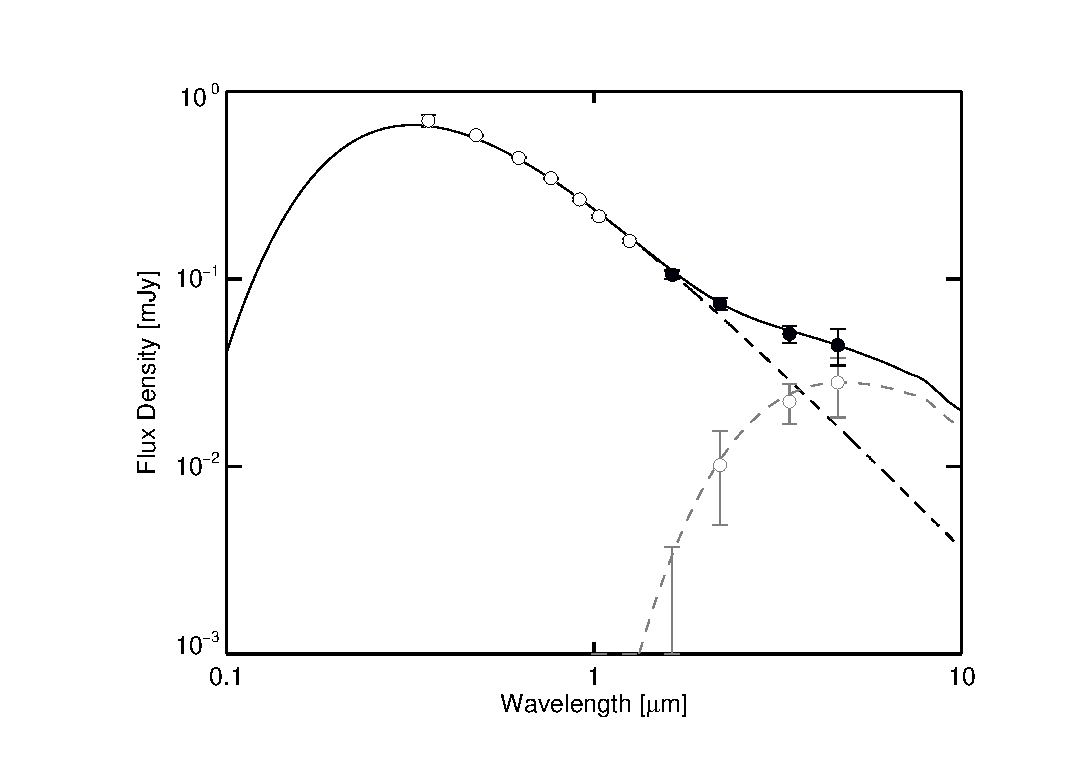
\includegraphics[width=7cm]{plots/wd1145p017_sed_astrosil.eps}
    \caption{SED of WD 1145+017. White data points show non-excess measurements, whilst black data points denote wavebands with excess emission. Greyed out data points are the excess flux at the wavelength of observation. Uncertainties are 1-$\sigma$. The solid black line is the combined white dwarf+disc model. The dashed black and grey lines denote the white dwarf and disc contributions to the total. \label{fig:wd1145p017_sed}}
\end{figure}

A least squares fit of the model with $a_{\rm min}$ as the only free parameter produces a best fit of $a_{\rm min} = 10.0^{+4.5}_{-3.2}~\mu$m, with a $\chi^{2}_{red}$ of 1.5 (three free parameters). The disc fractional luminosity ($L_{\rm dust}/L_{\rm WD}$) is calculated to be 3.2$\times10^{-3}$. The dust mass inferred from the model is 1.3$\times10^{19}$~g, about 1 per cent of the mass in fragments calculated by \cite{2015Natur.526..546V}. The grain size estimated here is consistent with that inferred for the dust from the flat transit depth between optical and near-infrared wavelengths. 


\section{Acknowledgments}
GZ thanks insightful discussions with Andrew Vanderburg \& Bryce Croll. JPM is supported by a UNSW Vice-Chancellor's Postdoctoral Fellowship. We thank the support staff at the AAO, who made the continued AAT+IRIS2 observations possible. 

Facilities: \facility{AAT}

\bibliographystyle{apj}
\bibliography{mybibfile}

\end{document}
